\documentclass[10pt]{article}
\usepackage[landscape]{geometry}
\usepackage{url}
\usepackage{multicol}
\usepackage{amsmath}
\usepackage{esint}
\usepackage{amsfonts}
\usepackage{tikz}
\usetikzlibrary{decorations.pathmorphing}
\usetikzlibrary{shapes,arrows}
\usetikzlibrary{positioning}
\usepackage{amsmath,amssymb}
\usepackage{chessfss}
\usepackage{colortbl}
\usepackage{xcolor}
\usepackage{mathtools}
\usepackage{amsmath,amssymb}
\usepackage{ragged2e}
\usepackage{bodegraph}
\usepackage{enumitem}
\usepackage{xcolor}
\usepackage{verbatim}

% Colors
\definecolor{bblue}{rgb}{0, 0.4470, 0.7410}
\definecolor{oorange}{rgb}{0.8500, 0.3250, 0.0980}
\definecolor{yyellow}{rgb}{0.9290 0.6940 0.1250}
\definecolor{ppurple}{rgb}{0.4940 0.1840 0.5560}
\definecolor{ggreen}{rgb}{0.4660 0.6740 0.1880}
\definecolor{bbblue}{rgb}{0.3010 0.7450 0.9330}

\makeatletter

\newcommand*\bigcdot{\mathpalette\bigcdot@{.5}}
\newcommand*\bigcdot@[2]{\mathbin{\vcenter{\hbox{\scalebox{#2}{$\m@th#1\bullet$}}}}}
\makeatother

\title{ML Cheat Sheet}
\usepackage[portuguese]{babel}
\usepackage[utf8]{inputenc}

\advance\topmargin-.8in
\advance\textheight3in
\advance\textwidth3in
\advance\oddsidemargin-1.5in
\advance\evensidemargin-1.5in
\parindent0pt
\parskip2pt
\newcommand{\hr}{\centerline{\rule{3.5in}{1pt}}}
\begin{document}
\begin{multicols*}{3}
\tikzstyle{mybox} = [draw=black, fill=white, very thick, rectangle, rounded corners, inner sep=10pt, inner ysep=10pt]
\tikzstyle{fancytitle} =[fill=black, text=white, font=\bfseries]
\tikzstyle{block} = [draw, rectangle, minimum height=3em, minimum width=6em, thick]
\tikzstyle{sum} = [draw, circle, node distance=1cm, thick]
\tikzstyle{input} = [coordinate]
\tikzstyle{output} = [coordinate]
\tikzstyle{pinstyle} = [pin edge={to-,thin,black}]

%------------ Modelação ---------------
\begin{tikzpicture}
\node [mybox] (box){%
    \small
    \begin{minipage}{0.3\textwidth}
    	LS: $\hat{\beta}_\mathrm{LS} = \underset{\beta}{\arg\min} \ ||y - X\beta||_2^2 \Rightarrow \hat{\beta}_\mathrm{LS} = (X^TX)^{-1}X^Ty$\\
        Polynomial: $f(x) = \sum_{k=0}^p \beta_kx^k$\\
        RBF: $G_k(x) = e^{-\frac{1}{2\sigma^2}||x-c^{(k)}||^2} \wedge w = (X^TX)^{-1}X^Ty \Rightarrow \\ \Rightarrow f(x) = \sum_{k=1}^p w_k G_k(x)$\\
        Ridge: $\hat{\beta}_\mathrm{ridge} = \underset{\beta}{\arg\min} \ ||y - X\beta||_2^2 + \lambda ||\beta||^2_2 \Rightarrow \\ \Rightarrow \hat{\beta}_\mathrm{ridge} = (X^TX + \lambda I)^{-1}X^Ty \rightarrow$ keep $\beta_k$ small\\
        Lasso: $\hat{\beta}_\mathrm{lasso} = \underset{\beta}{\arg\min} \ ||y - X\beta||_2^2 + \lambda ||\beta||_1 \rightarrow$ some $\beta_k = 0$\\
        Sparse: $\hat{\beta}_\mathrm{sparse} = \underset{\beta}{\arg\min} \ ||y - X\beta||_2^2 + \lambda \simeq \hat{\beta}_\mathrm{lasso}$
        \vspace{-0.3cm}
	\end{minipage}
};
\node[fancytitle, right=10pt] at (box.north west) {\texttt{Regression \& Regularization}};
\end{tikzpicture}

%------------ Optimization ---------------
\begin{tikzpicture}
\node [mybox] (box){%
    \small
    \begin{minipage}{0.3\textwidth}
        Gradient descent: $\theta^{(t+1)} = \theta^{(t)} - \eta \nabla_\theta J(\theta^{(t)})$\\
        Momentum technique: $v^{(t+1)} = \alpha v^{(t)} - \eta \nabla_\theta J(\theta^{(t)}) \wedge \theta^{(t+1)} = \theta^{(t)} + v^{(t+1)}, \ 0.5 \leq \alpha \leq 0.95 \rightarrow$ LP filtering\\
        Nesterov acc. grad.: $v^{(t+1)} = \alpha v^{(t)} - \eta \nabla_\theta J(\theta^{(t)} + \alpha v^{(t)}) \wedge \theta^{(t+1)} = \theta^{(t)} + v^{(t+1)}, \ 0.5 \leq \alpha \leq 0.95 \rightarrow $ better than MT\\
        Adaptive step size: {\scriptsize $\theta^{(t+1)}_i = \theta^{(t)}_i - \eta_i^{(t)} \frac{\partial J}{\partial \theta_i}(\theta^{(t)}) \wedge \\ \eta_i^{(t)} =  \begin{cases} u \eta_i^{(t-1)}, \ \mathrm{if} \ \frac{\partial J}{\partial \theta_i}(\theta^{(t)}) \times \frac{\partial J}{\partial \theta_i}(\theta^{(t - 1)}) > 0\\ d \eta_i^{(t - 1)}, \ \mathrm{otherwise} \end{cases}$} \hspace{-0.5cm} {\scriptsize, $u = 1.2 \wedge d = 0.8$}\\
        Newton method: $\theta^{(t+1)} = \theta^{(t)} - \left[H(\theta^{(t)})\right]^{-1} \nabla_\theta J(\theta^{(t)})$
        \vspace{-0.25cm}
    \end{minipage}
};
\node[fancytitle, right=10pt] at (box.north west) {\texttt{Optimization}};
\end{tikzpicture}

%------------ Evaluation & Generalization ---------------
\begin{tikzpicture}
\node [mybox] (box){%
    \small
    \begin{minipage}{0.3\textwidth}
        \textbf{Loss function}\\
        Regression: $L(y, \hat{y}) = (y-\hat{y})^2$\\
        Classification: $L(y, \hat{y}) = \begin{cases}0, \ y = \hat{y}\\ 1 , \ \mathrm{otherwise}\end{cases}\\$ or $L(y = i, \hat{y} = j) = L_{ij}$, where $L_{ii} = 0$\\
        \textbf{Risk}$\rightarrow \mathcal{R} = \mathrm{E}\{L(y, \hat{y}(x))\}$\\
        Regression: $\mathcal{R} = \int{\int{L(y, \hat{y}(x)) p(x, y)}}dxdy$\\
        Classification: $\mathcal{R} = \sum_y{\sum_x{L(y, \hat{y}(x)) P(x, y)}} = \\ = \sum_y\sum_{\hat{y}}L(y, \hat{y}) P(y, \hat{y})$\\
        \textbf{Empirical risk}$\rightarrow \mathcal{R}_\mathrm{e} = \frac{1}{n}\sum_{i = 1}^{n} L(y^{(i)}, f(x^{(i)}))$
        \vspace{-0.25cm}
    \end{minipage}
};
\node[fancytitle, right=10pt] at (box.north west) {\texttt{Evaluation \& Generalization}};
\end{tikzpicture}

%------------ Neural networks ---------------
\begin{tikzpicture}
\node [mybox] (box){%
    \small
    \begin{minipage}{0.3\textwidth}
        \textbf{Activation functions}\\
        $\mathrm{Sigmoid}_1$ (logistic): $g(s) = \frac{1}{1 + e^{-s}}$\\
        $\mathrm{Sigmoid}_2$ (arctangent): $g(s) = \arctan(x)$\\
        $\mathrm{Sigmoid}_3$ (softmax): $g(\mathbf{x})_i = \frac{e^{x_i}}{\sum_j e^{x_j}}\rightarrow$ output layer\\
        Linear unit: $g(s) = s \rightarrow$ output layer\\
        ReLU: $g(s) = s_+ = \max(0, s)\rightarrow$ recommended\\
        \textbf{MLP training}\\
        Total loss (cost): $\mathcal{C} = \sum_k L(y^{(k)}, \hat{y}^{(k)}) = \sum_k L^{(k)}$\\
        Loss (typical): $L(y, \hat{y}) = ||y-\hat{y}||_2^2$\\
        Min. $\mathcal{C}$: {\scriptsize $w_{ij}(t+1) = w_{ij}(t) + \Delta w_{ij}(t), \ \Delta w_{ij}(t) = -\eta \frac{\partial \mathcal{C}}{\partial w_{ij}}\Big|_{w(t)}$}\\
        Batch mode: $\Delta w_{ij}(t) = -\eta \sum_k\frac{\partial L^{(k)}}{\partial w_{ij}}$\\
        On-line mode (stoch. grad.): $\Delta w_{ij}(t) = -\eta \frac{\partial L^{(k)}}{\partial w_{ij}}$
        \vspace{-0.25cm}
    \end{minipage}
};
\node[fancytitle, right=10pt] at (box.north west) {\texttt{Neural networks}};
\end{tikzpicture}

\vspace{1.25cm}

%------------ Title ---------------
\begin{tikzpicture}
\node [] (box){%
    \huge
    \begin{minipage}{0.3\textwidth}
        \begin{center}
            \textbf{\texttt{ML} Cheat Sheet}\\
            \footnotesize \textcolor{bblue}{\texttt{[v2.0 - 13/11/22]}}
        \end{center}
    \end{minipage}
};
\end{tikzpicture}

%------------ Neural networks (cont.) ---------------
\begin{tikzpicture}
\node [mybox] (box){%
    \small
    \begin{minipage}{0.3\textwidth}
        
        \textbf{MLP architecture}\\
        Layer $\ell_1 = 1$: $s_q = w_{0q} + \sum_{i \in \mathrm{input}} w_{iq}x_i$, $z_q = g(s_q)$\\
        Layer $\ell_q > 1$: $s_q = w_{0q} + \sum_{i \in \mathrm{prev. layer}} w_{iq}z_i$, $z_q = g(s_q)$\\
        $\frac{\partial L}{\partial w_{pq}} = \frac{\partial L}{\partial s_q}\frac{\partial s_q}{\partial w_{pq}} = \varepsilon_q g(s_p) = \varepsilon_q z_p$, or $\varepsilon_qx_p$ if $i = j$\\
        {$\displaystyle \varepsilon_q = \frac{\partial L}{\partial s_q} = \sum_{j \in \mathrm{next \ell}} \frac{\partial L}{\partial s_j}\frac{\partial s_j}{\partial z_q}\frac{\partial z_q}{\partial s_q} = g'(s_q)\sum_{j \in \mathrm{next \ell}} w_{qj}\varepsilon_j$}\\
        \begin{minipage}{.5\textwidth}
		    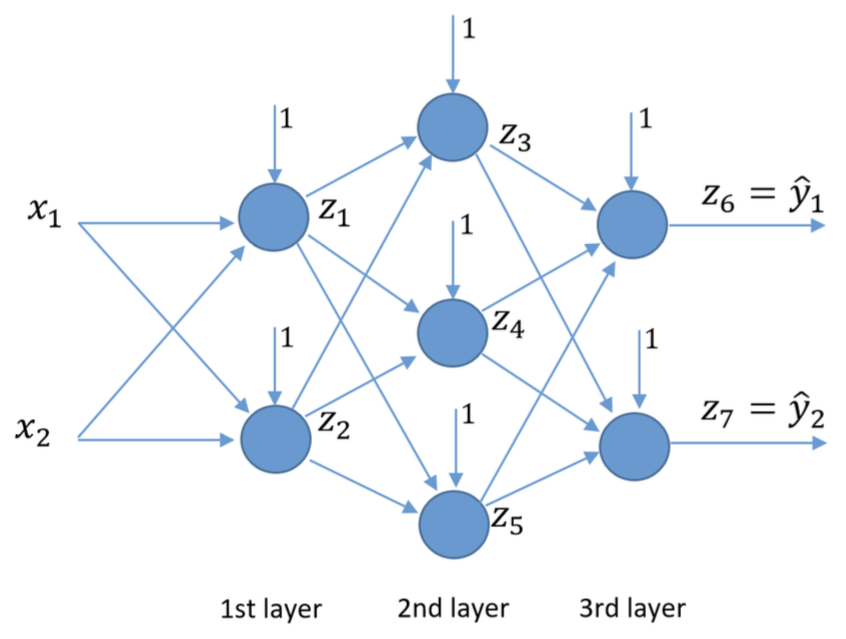
\includegraphics[scale=0.27]{figs/mlp.png}
        \end{minipage}\hfill
        \begin{minipage}{.5\textwidth}
		    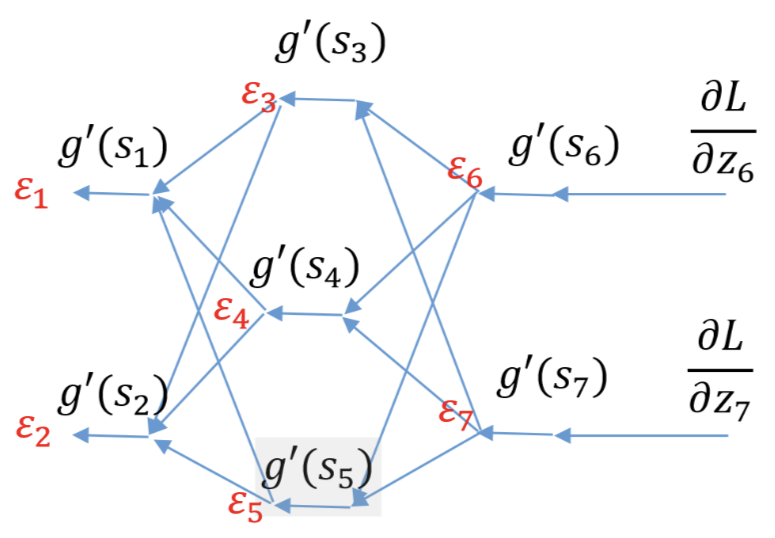
\includegraphics[scale=0.3]{figs/backprop.png}
        \end{minipage}\\
        Regression: output layer $\rightarrow g(s)$ linear, trained with SSE\\
        Classification: output layer $\rightarrow g(s)$ softmax/logistic, trained with negative log-likelihood (cross-entropy)\\
        \textbf{CNN acrchitecture}\\
        Convolutional $\ell$: convolve 3D array with kernels and $g$\\
        $s^\ell_{ij} = \sum_p\sum_q\sum_r h_{pqr}^\ell z^{\ell-1}_{i+p,j+q,0+r}$ (2D output), $z_{ij}^\ell = g(s_{ij}^\ell)$ and $h_{ijk}^\ell$ (3D kernel)\\
        Pooling: reduce size of 3D array, maximum/mean\\
        $z_{ijk}^\ell = \underset{p,q \in \{0,\dots, \Delta-1\}}{\max} \left\{z^{\ell - 1}_{\Delta i +p, \Delta j + q, k}\right\}$, $z^{\ell-1}_{i,j,k}$ (3D input)\\
        Fully connected $\ell$: when img representation is 1D array $\rightarrow$ often output layer
    \end{minipage}
};
\node[fancytitle, right=10pt] at (box.north west) {\texttt{Neural networks} (cont.)};
\end{tikzpicture}

%------------ Data classification ---------------
\begin{tikzpicture}
\node [mybox] (box){%
    \small
    \begin{minipage}{0.3\textwidth}
        Decision region: $\mathcal{R}_j = \{x \in \mathbb{R}^d: f(x) = \omega_j\}$, class $\omega_j$\\
        Confusion matrix: $P_{ij} = \mathrm{P}\{y = i, x \in \mathcal{R}_j\} = \int_{\mathcal{R}_j} p(x|y=i)P(y = i)dx$\\
        Rel. freq.: $\hat{P}_{ij} = \frac{N_{ij}}{\sum_{p=0}^{K-1} \sum_{q=0}^{K-1} N_{pq}}$\\
        Prob of error: $P(\mathrm{error}) = 1 - \sum_{i=0}^{K-1}P_{ii}$\\
        \textbf{Loss function}\\
        Binary: $L(y, \hat{y}) = \begin{cases} 0 \ \mathrm{if} \ \hat{y} = y\\ 1 \ \mathrm{otherwise}\end{cases}$\\
        General: $L(y = \omega_i, \hat{y} = \omega_j) = L_{ij}$, $L_{ij} > 0 \text{ for } i \neq j$\\
        \textbf{Ideal classifier (Bayes classifier)}\\
        Binary: $\hat{y} = \arg\underset{\omega \in \Omega}{\max} \ P(y = \omega | x)$\\
        General: {\footnotesize $f(x) =  \arg\underset{\omega \in \Omega}{\min} \ c_\omega(x)$, $c_\omega(x) = \sum_{y \in \Omega} L(y, \omega)P(y|x)$}\\
        \textbf{Bayes law}\\
        $P(y=i|x) = \frac{p(x|y=i)P(y=i)}{p(x)}$, $p(x) = \sum_{y\in \Omega}p(x|y)P(y)$\\
        \textbf{Na\"ive Bayes classifier}\\
        $\hat{y} =  \arg\underset{\omega \in \Omega}{\max} \prod_{i=1}^p p(x_i | y = k) \rightarrow$ features conditionally independent
        \vspace{-0.15cm}
    \end{minipage}
};
\node[fancytitle, right=10pt] at (box.north west) {\texttt{Data classification}};
\end{tikzpicture}

%------------ Linear classifiers ---------------
\begin{tikzpicture}
\node [mybox] (box){%
    \small
    \begin{minipage}{0.3\textwidth}
        Those whose decision boundaries are hyperplanes.\\
        One hot encoding: $y_i = \begin{cases} 1, \text{ if class $\omega_i$ occurs}\\ 0, \text{ otherwise}\end{cases}$\\
        Log-llh.: $\hat{\beta} = \arg\underset{\beta}{\max} \ \ell(\beta)$, $\ell(\beta) = \sum_{i=1}^n \log P(y^{(i)}, x^{(i)})$
        -- Logistic regression: $P(y = 1| x) = g(x^T\beta) \Rightarrow \ell(\beta) = \sum_{i = 1}^n \left\{y^{(i)}\log[g(x^{(i)T}\beta)] + (1- y^{(i)})\log[1 - g(x^{(i)T}\beta)]\right\}$\\
        -- Softmax: $P(y_i = 1| x, \beta) = \frac{e^{s_i}}{\sum_{c=0}^{K-1}e^{s_c}}, \ s_i = \sum_{j = 0}^p \beta_{ji}x_j \Rightarrow \ell(\beta) = \sum_{m = 1}^n \sum_{i = 0}^{K-1}\left\{y_i^{(m)}\log[\hat{y}_i^{(m)}]\right\}$
        \vspace{-0.25cm}
    \end{minipage}
};
\node[fancytitle, right=10pt] at (box.north west) {\texttt{Linear classifiers}};
\end{tikzpicture}

%------------ Support vector machines ---------------
\begin{tikzpicture}
\node [mybox] (box){%
    \small
    \begin{minipage}{0.3\textwidth}
        Hyperplane: $x \cdot w + b = 0 \Leftrightarrow x^Tw + b = 0$\\
        Distance to the origin: $\frac{|b|}{||w||_2}$\\
        Margin hyperplanes: $x^{(i)} \cdot w + b = \pm 1 , \ \mathrm{if} \ y^{(i)} = \pm 1$\\
        Margin: $\frac{2}{||w||_2}$\\
        Hard margin: linearly separable $\rightarrow \min \frac{1}{2}||w||^2_2 \rightarrow$ QP\\
        Soft margin: not lin. separable $\rightarrow \min \frac{1}{2}||w||^2_2 + C \sum_{i = 1}^n \xi_i$\\
        Hinge loss: $\xi_i = \max\left[0.1 - y^{(i)}(x^{(i)}\cdot w +b)\right]$\\
        Kernel trick: non lin. SVM $\rightarrow k(x^{(i)}, x^{(j)}) = \phi(x^{(i)}) \cdot \phi(x^{(j)})$, linear $x^{(i)T}x^{(j)}$, rbf $e^{-\frac{1}{2\sigma^2}||x^{(i)}-x^{(j)}||_2^2}$, poly $(x^{(i)T}x^{(j)}+a)^b$
        \vspace{-0.25cm}
    \end{minipage}
};
\node[fancytitle, right=10pt] at (box.north west) {\texttt{Support vector machines}};
\end{tikzpicture}

%------------ Decision Trees and Random Forest ---------------
\begin{tikzpicture}
\node [mybox] (box){%
    \small
    \begin{minipage}{0.3\textwidth}
    \emph{A posteriori} dist.: $P(k|m) = \frac{1}{\#\mathcal{T}_m} \sum_{x^{(i)} \in \mathcal{T}_m} I(y^{(i)} = k)$, node $m$, indicator function $I(\cdot)$\\
    $m$ is a leaf $\Rightarrow$ most probable label is $\hat{k} = \arg\underset{k}{\max} \ P(k|m)$\\
    \textbf{Impurity}\\
    Misclass. error: $i(m) = 1 - \underset{k}{\max} \ P(k|m) = 1 - P(\hat{k}(m)|m)$\\
    Entropy: $i(m) = -\sum_{k=1}^K P(k|m)\log_2 P(k|m)$\\
    Gini index: $i(m) = -\sum_{k=1}^K P(k|m)(1 - P(k|m))$\\
    Tree training: minimize $I(T) = \sum_{m \in \tilde{T}}P(m)i(m)$\\
    Impurity drop: $\Delta I = i(m) - \sum_{s \in S}\frac{p(s)}{p(m)}i(s)$, $m$ node is splitted into $s \in S$ children nodes\\
    ID3: impurity criterion = entropy, stop criterion = when each leaf is pure\\
    Bootstrap aggregation = bagging: regression -- averaging all functions learned in each bootstraped data set; classification -- averaging the \emph{a posteriori} learned probabilities in each data set\\
    Random forest: ensemble of tree classifiers trained with bagging
    \vspace{-0.25cm}
    \end{minipage}
};
\node[fancytitle, right=10pt] at (box.north west) {\texttt{Decision Trees and Random Forest}};
\end{tikzpicture}

\scriptsize
\raggedleft
Based on Machine Learning Slides\\
Transcribed, edited and adapted by\\
João Marafuz Gaspar -- 96240 \\
IST, 2022
\end{multicols*}
\end{document}

